\documentclass[a4paper,12pt]{article}
\usepackage[brazil, english]{babel}
\usepackage[utf8]{inputenc}
\usepackage[T1]{fontenc}
\usepackage{geometry}
\usepackage{setspace}
\usepackage{titlesec}
\usepackage{hyperref}
\usepackage{graphicx}
\usepackage{caption}
\usepackage{subcaption}
\usepackage{fancyhdr}
\usepackage{xcolor}
\usepackage{amsmath, amssymb, bm}
\usepackage{mathtools}
\usepackage{cancel}
\usepackage{tikz}
\usepackage{newunicodechar}
\newunicodechar{∘}{\circ}

%%%%%%%%%%%%%%%%%%%%%%%%%%%%%%%%%%%%%%%%%%%%%%%%%%
% These are some new commands that may be useful 
% for paper writing in general. If other new commands
% are needed for your specific paper, please feel 
% free to add here. 
%
% The currently available commands are organized in: 
% 1) Systems
% 2) Quantities
% 3) Energies and units
% 4) particle species
% 5) Colors package
% 6) hyperlink
%%%%%%%%%%%%%%%%%%%%%%%%%%%%%%%%%%%%%%%%%%%%%%%%%%

\usepackage{amsmath}
\usepackage{amssymb}
\usepackage{upgreek}
\usepackage{multirow}
\usepackage{setspace}% http://ctan.org/pkg/setspace
\usepackage{fancyhdr}
\usepackage{datetime}

% 1) SYSTEMS
\newcommand{\btc}               {\textbf{BTC}}
\newcommand{\btcspace}          {\textbf{BTC} }
\newcommand{\pow}               {\textbf{PoW}}

% 4) definition to references, biblatex and hyperlink
\usepackage[backend=bibtex, 
style=nature,  %style reference.
sorting=none,
firstinits=true %first name abbreviate
]{biblatex}

\usepackage{hyperref}
\hypersetup{
    colorlinks=true, %set "true" if you want colored links
    linktoc=all,     %set to "all" if you want both sections and subsections linked
    linkcolor=blue,  %choose some color if you want links to stand out
    citecolor= blue, % color of \cite{} in the text.
    urlcolor  = blue, % color of the link for the paper in references.
}

% 5) Tikz and figures
\usepackage{epsfig}
\usepackage{lmodern}
\usepackage{mathtools}
\usepackage[utf8]{luainputenc}
\usepackage{xspace}
\usepackage{tikz}
\usepackage{pgfplots}
\pgfplotsset{compat=newest}

\usetikzlibrary{positioning}
\usepackage{subcaption}

% 6) colors:
\usepackage{xcolor}
\definecolor{ao(english)}{rgb}{0.0, 0.5, 0.0} % dark green

% 7) Add lines numbers
%\usepackage{lineno}

% add pdf file to thesis:
\usepackage{pdfpages}

\hypersetup{
    colorlinks=true,% make the links colored
    linkcolor=blue
}

\usepackage{setspace}
\addbibresource{bibliography.bib}

\newcommand{\printingbibliography}{%

    \pagestyle{myheadings}
    \markright{}
    \sloppy
    \printbibliography[heading=bibintoc, % add to table of contents
                   title=Refer\^encias % Chapter name
                  ]
    \fussy%
}
\PassOptionsToPackage{table}{xcolor}

\pagestyle{fancy}
\fancyhf{}
\renewcommand{\headrulewidth}{0pt}
\fancyhead[R]{\thepage}

\geometry{a4paper,top=30mm,bottom=20mm,left=30mm,right=20mm}

\titleformat*{\section}{\bfseries\large}
\titleformat*{\subsection}{\bfseries\normalsize}

\title{ \textbf{\large Eletromagnetismo I }}
\author{Andr\'e V. Silva}
\date{\today}

\begin{document}

\maketitle

\begin{center}
    \textbf{Prof. Bruno Moraes - 2024-2}\
    \textbf{Guia de Estudo 1: Revisão Matemática}
    \end{center}
    
    * A numeração dos exercícios do Griffiths propostos correspondem à 4a edição em inglês.\\
    
    \begin{center}
    \colorbox{yellow}{\textbf{Resolu\c{c}\~ao de Exerc\'icios}}
    \end{center}
    
    \begin{enumerate}
    \item Griffiths \textbf{Seção 1.1} - \colorbox{green}{1.5} 
    \item Griffiths \textbf{Seção 1.2} - \colorbox{green}{1.13(*)}, \colorbox{green}{1.16(*)}, \colorbox{green}{1.19}, \colorbox{green}{1.21}, \colorbox{green}{1.22(a-b)}
    \item Griffiths \textbf{Seção 1.3} - \colorbox{green}{1.36}
    \item Griffiths \textbf{Seção 1.4} - \colorbox{green}{1.38(*)}, \colorbox{green}{1.42}
    \item Griffiths \textbf{Seção 1.5} - \colorbox{green}{1.44}, \colorbox{green}{1.45}, \colorbox{green}{1.46}, 1.47. 1.48, 1.49
    \item Griffiths \textbf{Seção 1.6} - 1.51, 1.52
    \item Problemas adicionais - 1.62(*), 1.63(*)
    \end{enumerate}

\section*{Problema 1.5 Griffiths - Resolu\c{c}\~ao}

O produto vetorial triplo: $\textrm{\textbf{A}}\times\textrm{\textbf{B}}\times\textrm{\textbf{C}}$
ser simplificado pela express\~ao \textbf{BAC} - \textbf{CAB}:

\begin{equation}
    \textbf{A}\times(\textbf{B}\times\textbf{C}) =  \textbf{B}(\textbf{A}\cdot\textbf{C}) - \textbf{C}(\textbf{A}\cdot\textbf{B})
\end{equation}

Com isso, podemos notar que:

\begin{equation}
    (\textbf{A}\times\textbf{B})\times\textbf{C} = -\textbf{C}\times(\textbf{A}\times\textbf{B}) = -\textbf{A}(\textbf{B}\cdot\textbf{C}) + \textbf{B}(\textbf{A}\cdot\textbf{C})
\end{equation}

Vamos provar \textbf{BAC} - \textbf{CAB} escrevendo explicitamente ambos os lados em termos de suas componentes:\\

Primeramente, definindo \textbf{A} $= (\textrm{A}_{x}, \textrm{A}_{y}, \textrm{A}_{z}$), \textbf{B} $= (\textrm{B}_{x}, \textrm{B}_{y}, \textrm{B}_{z}$) 
e \textbf{C} $= (\textrm{C}_{x}, \textrm{C}_{y}, \textrm{C}_{z}$)\\

Lado esquerdo da equa\c{c}\~ao (1) parte por parte:

\begin{equation}
    \mathbf{B} \times \mathbf{C} =
\begin{vmatrix}
\mathbf{i} & \mathbf{j} & \mathbf{k} \\
B_x & B_y & B_z \\
C_x & C_y & C_z
\end{vmatrix} =
(B_yC_z - B_zC_y)\mathbf{i} +
(B_zC_x - B_xC_z)\mathbf{j} +
(B_xC_y - B_yC_x)\mathbf{k}
\end{equation}


\begin{equation}
\mathbf{A} \times (\mathbf{B} \times \mathbf{C}) =
\begin{vmatrix}
\mathbf{i} & \mathbf{j} & \mathbf{k} \\
A_x & A_y & A_z \\
(B_yC_z - B_zC_y) & (B_zC_x - B_xC_z) & (B_xC_y - B_yC_x)
\end{vmatrix}
\end{equation}

\begin{equation}
    \begin{aligned}
    \mathbf{A} \times (\mathbf{B} \times \mathbf{C}) = \left[ A_y(B_xC_y - B_yC_x) - A_z(B_zC_x - B_xC_z) \right] \mathbf{i} \\ +
    \left[A_z(B_yC_z - B_zC_y) - A_x(B_xC_y - B_yC_x) \right] \mathbf{j}\\ +
    \left[ A_x(B_zC_x - B_xC_z) - A_y(B_yC_z - B_zC_y) \right] \mathbf{k}.
\end{aligned}
\end{equation}\\


A expressão \( \mathbf{B}(\mathbf{A} \cdot \mathbf{C}) \) em termos das componentes \( \mathbf{i}, \mathbf{j}, \mathbf{k} \) é dada por:

Seja \( \mathbf{B} = B_x \mathbf{i} + B_y \mathbf{j} + B_z \mathbf{k} \) e o produto escalar \( \mathbf{A} \cdot \mathbf{C} = A_x C_x + A_y C_y + A_z C_z \), então:

\begin{equation}
\mathbf{B} (\mathbf{A} \cdot \mathbf{C}) = (B_x \mathbf{i} + B_y \mathbf{j} + B_z \mathbf{k}) (A_x C_x + A_y C_y + A_z C_z)
\end{equation}

Ou, expandindo a expressão, temos:

\begin{equation}
    \begin{aligned}
\mathbf{B} (\mathbf{A} \cdot \mathbf{C}) = \left( B_x (A_x C_x + A_y C_y + A_z C_z) \right) \mathbf{i}\\
             + \left( B_y (A_x C_x + A_y C_y + A_z C_z) \right) \mathbf{j}\\
             + \left( B_z (A_x C_x + A_y C_y + A_z C_z) \right) \mathbf{k}
\end{aligned}
\end{equation}

A expressão \( \mathbf{C}(\mathbf{A} \cdot \mathbf{B}) \) em termos das componentes \( \mathbf{i}, \mathbf{j}, \mathbf{k} \) é dada por:

Seja \( \mathbf{C} = C_x \mathbf{i} + C_y \mathbf{j} + C_z \mathbf{k} \) e o produto escalar \( \mathbf{A} \cdot \mathbf{B} = A_x B_x + A_y B_y + A_z B_z \), então:

\begin{equation}
\mathbf{C} (\mathbf{A} \cdot \mathbf{B}) = (C_x \mathbf{i} + C_y \mathbf{j} + C_z \mathbf{k}) (A_x B_x + A_y B_y + A_z B_z)
\end{equation}

Ou, expandindo a expressão, temos:

\begin{equation}
    \begin{aligned}
\mathbf{C} (\mathbf{A} \cdot \mathbf{B}) = \left( C_x (A_x B_x + A_y B_y + A_z B_z) \right) \mathbf{i}\\
        + \left( C_y (A_x B_x + A_y B_y + A_z B_z) \right) \mathbf{j} \\
        + \left( C_z (A_x B_x + A_y B_y + A_z B_z) \right) \mathbf{k}
\end{aligned}
\end{equation}

Ent\~ao


\begin{equation}
    \begin{aligned}
\mathbf{B} (\mathbf{A} \cdot \mathbf{C}) - \mathbf{C} (\mathbf{A} \cdot \mathbf{B}) = & \, \Big( B_x (A_x C_x + A_y C_y + A_z C_z) - C_x (A_x B_x + A_y B_y + A_z B_z) \Big) \mathbf{i} \\
& + \Big( B_y (A_x C_x + A_y C_y + A_z C_z) - C_y (A_x B_x + A_y B_y + A_z B_z) \Big) \mathbf{j} \\
& + \Big( B_z (A_x C_x + A_y C_y + A_z C_z) - C_z (A_x B_x + A_y B_y + A_z B_z) \Big) \mathbf{k}.
    \end{aligned}
\end{equation}

\begin{equation}
    \begin{aligned}
\mathbf{B} (\mathbf{A} \cdot \mathbf{C}) - \mathbf{C} (\mathbf{A} \cdot \mathbf{B}) = & \, \Big( \cancel{A_x B_x C_x} + A_y B_x C_y + A_z B_x C_z -  \cancel{A_x B_x C_x}  - A_y C_x B_y - A_z C_xB_z \Big) \mathbf{i} \\
& + \Big(  A_x B_y C_x + \cancel{A_y B_y C_y} + A_z B_y C_z  - A_x C_y B_x - \cancel{A_y B_y C_y} - A_z C_y B_z \Big) \mathbf{j} \\
& + \Big(  A_x B_z C_x + A_y B_z C_y + \cancel{A_z B_z C_z} - A_x C_z B_x - A_y B_y C_z - \cancel{A_z B_z C_z} \Big) \mathbf{k}.
    \end{aligned}
\end{equation}

\begin{equation}
    \begin{aligned}
\mathbf{B} (\mathbf{A} \cdot \mathbf{C}) - \mathbf{C} (\mathbf{A} \cdot \mathbf{B}) = & \, \Big(A_y B_x C_y + A_z B_x C_z - A_y C_x B_y - A_z C_xB_z \Big) \mathbf{i} \\
& + \Big(  A_x B_y C_x + A_z B_y C_z  - A_x C_y B_x - A_z C_y B_z \Big) \mathbf{j} \\
& + \Big(  A_x B_z C_x + A_y B_z C_y - A_x C_z B_x - A_y B_y C_z \Big) \mathbf{k}.
    \end{aligned}
\end{equation}

\begin{equation}
\boxed{
    \begin{aligned}
\mathbf{B} (\mathbf{A} \cdot \mathbf{C}) - \mathbf{C} (\mathbf{A} \cdot \mathbf{B}) = & \, \Big[A_y (B_x C_y -B_y C_x ) - A_z (B_z C_x - B_x C_z) \Big] \mathbf{i} \\
& + \Big[ A_z (B_y C_z - C_y B_z) - A_x (B_x C_y  - B_y C_x)     \Big] \mathbf{j} \\
& + \Big[  A_x(B_z C_x - B_x C_z)  - A_y (B_y C_z - B_z C_y)   \Big] \mathbf{k}.
    \end{aligned}
}
\end{equation}


\begin{equation}
    \boxed{
    \begin{aligned}
    \mathbf{A} \times (\mathbf{B} \times \mathbf{C}) = \Big[ A_y(B_xC_y - B_yC_x) - A_z(B_zC_x - B_xC_z) \Big] \mathbf{i} \\ +
    \Big[A_z(B_yC_z - B_zC_y) - A_x(B_xC_y - B_yC_x) \Big] \mathbf{j}\\ +
    \Big[ A_x(B_zC_x - B_xC_z) - A_y(B_yC_z - B_zC_y) \Big] \mathbf{k}.
\end{aligned}
    }
\end{equation}\\

Portanto,

\begin{equation}
    \mathbf{A} \times (\mathbf{B} \times \mathbf{C}) =\mathbf{B} (\mathbf{A} \cdot \mathbf{C}) - \mathbf{C} (\mathbf{A} \cdot \mathbf{B}) \hspace{3cm} \blacksquare
\end{equation}


Ambos os termos concordam!


\section*{Problema 1.13 Griffiths - Resolu\c{c}\~ao}

Seja \(\mathbf{r}\) o vetor separação de um ponto fixo \((x', y', z')\) até o ponto \((x, y, z)\), e \(r\) o módulo de \(\mathbf{r}\). Mostre que:

\begin{enumerate}
    \item[(a)] \(\nabla (r^2) = 2\mathbf{r}\),
    \item[(b)] \(\nabla \left(\frac{1}{r}\right) = -\frac{\hat{\mathbf{r}}}{r^2}\), onde \(\hat{\mathbf{r}} = \frac{\mathbf{r}}{r}\) é o vetor unitário,
    \item[(c)] A fórmula geral para \(\nabla (r^n)\)?
\end{enumerate}


Seja o vetor separação \(\mathbf{r}\), definido como:

\begin{equation}
\mathbf{r} = (x - x', y - y', z - z'),
\end{equation}

e seu módulo \(r = |\mathbf{r}| = \sqrt{(x - x')^2 + (y - y')^2 + (z - z')^2}\).

\subsection*{Parte (a)}

Queremos mostrar que:
\begin{equation}
\nabla (r^2) = 2\mathbf{r}.
\end{equation}

Sabemos que:
\begin{equation}
r^2 = \mathbf{r} \cdot \mathbf{r} = (x - x')^2 + (y - y')^2 + (z - z')^2.
\end{equation}

O gradiente em coordenadas cartesianas é dado por:
\begin{equation}
\nabla f = \left( \frac{\partial f}{\partial x}, \frac{\partial f}{\partial y}, \frac{\partial f}{\partial z} \right).
\end{equation}

Cálculo das derivadas parciais:
\begin{equation}
\frac{\partial (r^2)}{\partial x} = 2(x - x'), \quad
\frac{\partial (r^2)}{\partial y} = 2(y - y'), \quad
\frac{\partial (r^2)}{\partial z} = 2(z - z').
\end{equation}

Logo:
\begin{equation}
\nabla (r^2) = \left( 2(x - x'), 2(y - y'), 2(z - z') \right) = 2\mathbf{r}.
\end{equation}

\subsection*{Parte (b)}

Queremos mostrar que:
\begin{equation}
\nabla \left(\frac{1}{r}\right) = -\frac{\hat{\mathbf{r}}}{r^2},
\end{equation}
onde \(\hat{\mathbf{r}} = \frac{\mathbf{r}}{r}\) é o vetor unitário.

Sabemos que:
\begin{equation}
\frac{1}{r} = \left[ (x - x')^2 + (y - y')^2 + (z - z')^2 \right]^{-1/2}.
\end{equation}

Aplicando a regra da cadeia:
\begin{equation}
\nabla \left(\frac{1}{r}\right) = \nabla \left[ (r^2)^{-1/2} \right] = -\frac{1}{2} (r^2)^{-3/2} \nabla (r^2).
\end{equation}

Da parte (a), \(\nabla (r^2) = 2\mathbf{r}\). Substituímos:
\begin{equation}
\nabla \left(\frac{1}{r}\right) = -\frac{1}{2} (r^2)^{-3/2} (2\mathbf{r}) = -\frac{\mathbf{r}}{r^3}.
\end{equation}

Escrevendo em termos de \(\hat{\mathbf{r}}\):
\begin{equation}
\nabla \left(\frac{1}{r}\right) = -\frac{\hat{\mathbf{r}}}{r^2}.
\end{equation}

\subsection*{Parte (c)}

Queremos determinar a fórmula geral para:
\begin{equation}
\nabla (r^n).
\end{equation}

Sabemos que \(r^n = (r^2)^{n/2}\). Aplicando a regra da cadeia:
\begin{equation}
\nabla (r^n) = \frac{d}{dr}(r^n) \nabla r.
\end{equation}

A derivada em relação a \(r\) é:
\begin{equation}
\frac{d}{dr}(r^n) = n r^{n-1}.
\end{equation}

Como 

\(\nabla r = \Big(\hat{\mathbf{x}}\frac{\partial}{\partial x}, \hat{\mathbf{y}}\frac{\partial}{\partial y}, \hat{\mathbf{z}}\frac{\partial }{\partial z} \Big) r  = \frac{\mathbf{r}}{r}\), 


obtemos:
\begin{equation}
\nabla (r^n) = n r^{n-1} \frac{\mathbf{r}}{r} = n r^{n-1} \hat{\mathbf{r}}.
\end{equation}

\subsection*{Resultado Final}

(a) \(\nabla (r^2) = 2\mathbf{r}\),

(b) \(\nabla \left(\frac{1}{r}\right) = -\frac{\hat{\mathbf{r}}}{r^2}\),

(c) \(\nabla (r^n) = n r^{n-1} \hat{\mathbf{r}}\).


\section*{Problema 1.16 Griffiths - Resolu\c{c}\~ao}

\begin{center}
\begin{tikzpicture}
    % Ponto de origem
    \node[circle, fill=red, inner sep=1.5pt] (O) at (0,0) {};
    
    % Setas divergentes
    \draw[->, thick] (O) -- (0,0.5) node[midway, above] {};
    \draw[->, thick] (0,0.6) -- (0,1) node[midway, above] {};
    \draw[->, thick] (0,1.1) -- (0,1.6) node[midway, above] {};

    \draw[->, thick] (O) -- (0,-0.5) node[midway, above] {};
    \draw[->, thick] (0,-0.6) -- (0,-1) node[midway, above] {};
    \draw[->, thick] (0,-1.1) -- (0,-1.6) node[midway, above] {};

    \draw[->, thick] (O) -- (0.4,0.4) node[midway, above] {};
    \draw[->, thick] (0.41,0.41) -- (0.8,0.8) node[midway, above] {};
    \draw[->, thick] (0.81,0.81) -- (1.2,1.2) node[midway, above] {};

    \draw[->, thick] (O) -- (-0.4,0.4) node[midway, above] {};
    \draw[->, thick] (-0.41,0.41) -- (-0.8,0.8) node[midway, above] {};
    \draw[->, thick] (-0.81,0.81) -- (-1.2,1.2) node[midway, above] {};

    \draw[->, thick] (O) -- (0.4,-0.4) node[midway, above] {};
    \draw[->, thick] (0.41,-0.41) -- (0.8,-0.8) node[midway, above] {};
    \draw[->, thick] (0.81,-0.81) -- (1.2,-1.2) node[midway, above] {};

    \draw[->, thick] (O) -- (-0.4,-0.4) node[midway, above] {};
    \draw[->, thick] (-0.41,-0.41) -- (-0.8,-0.8) node[midway, above] {};
    \draw[->, thick] (-0.81,-0.81) -- (-1.2,-1.2) node[midway, above] {};

    \draw[->, thick] (O) -- (0.5,0) node[midway, below] {};
    \draw[->, thick] (0.51,0) -- (1,0) node[midway, below] {};
    \draw[->, thick] (1.1,0) -- (1.5,0) node[midway, below] {};

    \draw[->, thick] (O) -- (-0.5,0) node[midway, below] {};
    \draw[->, thick] (-0.51,0) -- (-1,0) node[midway, below] {};
    \draw[->, thick] (-1.1,0) -- (-1.5,0) node[midway, below] {};



\end{tikzpicture}
\end{center}

Esboce a função vetorial 
\begin{equation}
\mathbf{v} = \frac{\hat{\mathbf{r}}}{r^2},
\end{equation}
e calcule sua divergência. O resultado pode surpreendê-lo... você consegue explicá-lo?

A função vetorial fornecida é 
\begin{equation}
\mathbf{v} = \frac{\hat{\mathbf{r}}}{r^2},
\end{equation}
onde:
\begin{itemize}
    \item \( \hat{\mathbf{r}} \) é o vetor unitário na direção radial;
    \item \( r = \sqrt{x^2 + y^2 + z^2} \) é a distância até a origem.
\end{itemize}

---

\subsection*{Cálculo da divergência}

A divergência em coordenadas cartesianas para um campo vetorial puramente radial é dada por:

\begin{equation}
\nabla \cdot \mathbf{v} = \frac{\partial}{\partial x}\left( \frac{x}{r^3}\right) + \frac{\partial}{\partial y}\left( \frac{y}{r^3}\right) + \frac{\partial}{\partial z}\left( \frac{z}{r^3}\right)
\end{equation}

\begin{equation}
    \nabla \cdot \mathbf{v} = \frac{\partial}{\partial x}\left[x(x^2+y^2+z^2)^{-\frac{3}{2}}\right] + \frac{\partial}{\partial y}\left[x(x^2+y^2+z^2)^{-\frac{3}{2}}\right] + \frac{\partial}{\partial z}\left[z(x^2+y^2+z^2)^{-\frac{3}{2}}\right]
\end{equation}

Para a componente \( x \), temos:

\begin{equation}
    \frac{\partial}{\partial x}\left[x(x^2+y^2+z^2)^{-\frac{3}{2}}\right] = (x^2+y^2+z^2)^{-\frac{3}{2}} + \left(-\frac{3}{2}\right)(x^2+y^2+z^2)^{-\frac{5}{2}}\left(2x^2\right)
\end{equation}

\begin{equation}
    \frac{\partial}{\partial x}\left[x(x^2+y^2+z^2)^{-\frac{3}{2}}\right] = r^{-3} - 3r^{-5}\left(x^2\right)
\end{equation}

Analogo para y e z:

\begin{equation}
    \frac{\partial}{\partial y}\left[x(x^2+y^2+z^2)^{-\frac{3}{2}}\right] = r^{-3} - 3r^{-5}\left(y^2\right)
\end{equation}

\begin{equation}
    \frac{\partial}{\partial z}\left[x(x^2+y^2+z^2)^{-\frac{3}{2}}\right] = r^{-3} - 3r^{-5}\left(z^2\right)
\end{equation}

Ent\~ao:

\begin{equation}
    \nabla \cdot \mathbf{v} = 3r^{-3} -3r^{-5}\left(x^2+y^2+z^2\right)
\end{equation}

como $r^2 = x^2 + y^2 + z^2$:

\begin{equation}
    \nabla \cdot \mathbf{v} = 3r^{-3} - 3r^{-5}r^2 = 3r^{-3} - 3r^{-3} = 0 
\end{equation}

\subsection*{Explicação do resultado surpreendente}

Embora a divergência seja \( 0 \) em todos os pontos onde \( r \neq 0 \), o campo possui uma singularidade no 
ponto \( r = 0 \), onde o módulo de \( \mathbf{v} \) diverge. Esse comportamento pode ser explicado utilizando 
o conceito de função delta de Dirac. 

A divergência completa pode ser escrita como:
\begin{equation}
\nabla \cdot \mathbf{v} = 4\pi \delta^3(\mathbf{r}),
\end{equation}
onde \( \delta^3(\mathbf{r}) \) é a função delta de Dirac em três dimensões. Isso indica que toda a "fonte" 
do campo está concentrada no ponto \( r = 0 \). A singularidade pode ser tratada utilizando a função delta de Dirac, 
que é uma função generalizada (ou distribuição) que permite modelar distribuições de carga ou fluxo concentrado em 
pontos específicos.

---

\section*{Conclusão}

O campo vetorial \( \mathbf{v} = \frac{\hat{\mathbf{r}}}{r^2} \) possui divergência igual a \( 0 \) em todos os pontos do espaço, 
exceto na origem, onde ocorre uma singularidade representada pela função delta de Dirac.

\newpage
\section*{Problema 1.19 Griffiths - Resolu\c{c}\~ao}

\begin{figure}[!h]
    \centering
\begin{tikzpicture}
    % Desenho do círculo
    \draw[thick, dashed] (0,0) circle (3);
    
    % Eixos coordenados
    \draw[->, thick, blue] (-4,0) -- (4,0) node[anchor=west] {$x$};
    \draw[->, thick, blue] (0,-4) -- (0,4) node[anchor=south] {$y$};
    \draw[->, thick, blue] (0,0) -- (-2,-3) node[anchor=north] {$z$};

    % Ponto A e vetor velocidade em A
    \filldraw[red] (-3,0) circle (2pt) node[anchor=north east] {$A$};
    \draw[->, thick] (-3,0) -- (-3,1) node[anchor=east] {$\mathbf{v}$};

    % Ponto B e vetor velocidade em B
    \filldraw[red] (-2.12,2.12) circle (2pt) node[anchor=south east] {$B$};
    \draw[->, thick] (-2.12,2.12) -- (-1.12,3.12) node[anchor=west] {$\mathbf{v}$};

    % Vetores em outros pontos
    \draw[->, thick] (2.12,2.12) -- (3.12,1.12) node[anchor=west] {$\mathbf{v}$};
    \draw[->, thick] (2.12,-2.12) -- (1.12,-3.12) node[anchor=east] {$\mathbf{v}$};
    \draw[->, thick] (-2.12,-2.12) -- (-3.12,-1.12) node[anchor=east] {$\mathbf{v}$};
\end{tikzpicture}
\caption{Rotação do vetor \textbf{v} ao movermos o ponto \textbf{A} para o ponto \textbf{B}.}
\label{fig:circle_diagram}
\end{figure}

Ao movermos do ponto $A$ para o ponto $B$ (como visto na Figure~\ref{fig:circle_diagram}), $x$ aumenta, $y$ aumenta, $v_x$ aumenta 
e $v_y$ diminui. Assim, temos que $\partial v_x / \partial y > 0$, enquanto $\partial v_y / \partial y < 0$. 
No círculo, $v_z = 0$ e não há dependência de $z$, portanto, a Eq. 1.41 nos dá:

\begin{equation}
\nabla \times \mathbf{v} = \hat{\mathbf{z}} \left( \frac{\partial v_y}{\partial x} - \frac{\partial v_x}{\partial y} \right)
\end{equation}

e aponta na \fbox{direção negativa de $z$} (para dentro da página), como a regra da mão direita sugere. 
Escolha quaisquer outros pontos próximos no círculo e você chegará à mesma conclusão.

\section*{Problema 1.21 Griffiths - Resolu\c{c}\~ao}

\begin{itemize}
    \item[(i)] 
    \begin{equation}
    \nabla (fg) = \frac{\partial (fg)}{\partial x} \hat{\mathbf{x}} + \frac{\partial (fg)}{\partial y} \hat{\mathbf{y}} + \frac{\partial (fg)}{\partial z} \hat{\mathbf{z}}
    \end{equation}
    \begin{equation}
    = \left( f \frac{\partial g}{\partial x} + g \frac{\partial f}{\partial x} \right) \hat{\mathbf{x}} + \left( f \frac{\partial g}{\partial y} + g \frac{\partial f}{\partial y} \right) \hat{\mathbf{y}} + \left( f \frac{\partial g}{\partial z} + g \frac{\partial f}{\partial z} \right) \hat{\mathbf{z}}
    \end{equation}
    \begin{equation}
    = f \left( \frac{\partial g}{\partial x} \hat{\mathbf{x}} + \frac{\partial g}{\partial y} \hat{\mathbf{y}} + \frac{\partial g}{\partial z} \hat{\mathbf{z}} \right) + g \left( \frac{\partial f}{\partial x} \hat{\mathbf{x}} + \frac{\partial f}{\partial y} \hat{\mathbf{y}} + \frac{\partial f}{\partial z} \hat{\mathbf{z}} \right)
    \end{equation}
    \begin{equation}
    = f (\nabla g) + g (\nabla f). \quad \text{qed}
    \end{equation}

    \item[(iv)]
    \begin{equation}
    \nabla \cdot (\mathbf{A} \times \mathbf{B}) = \frac{\partial}{\partial x} (A_y B_z - A_z B_y) + \frac{\partial}{\partial y} (A_z B_x - A_x B_z) + \frac{\partial}{\partial z} (A_x B_y - A_y B_x)
    \end{equation}
    \begin{equation}
    = A_y \frac{\partial B_z}{\partial x} + B_z \frac{\partial A_y}{\partial x} - A_z \frac{\partial B_y}{\partial x} - B_y \frac{\partial A_z}{\partial x} 
    \end{equation}
    \begin{equation}
    + A_z \frac{\partial B_x}{\partial y} + B_x \frac{\partial A_z}{\partial y} - A_x \frac{\partial B_z}{\partial y} - B_z \frac{\partial A_x}{\partial y}
    \end{equation}
    \begin{equation}
    + A_x \frac{\partial B_y}{\partial z} + B_y \frac{\partial A_x}{\partial z} - A_y \frac{\partial B_x}{\partial z} - B_x \frac{\partial A_y}{\partial z}
    \end{equation}
    \begin{equation}
    = B_x \left( \frac{\partial A_z}{\partial y} - \frac{\partial A_y}{\partial z} \right) + B_y \left( \frac{\partial A_x}{\partial z} - \frac{\partial A_z}{\partial x} \right) + B_z \left( \frac{\partial A_y}{\partial x} - \frac{\partial A_x}{\partial y} \right)
    \end{equation}
    \begin{equation}
    - A_y \left( \frac{\partial B_z}{\partial x} - \frac{\partial B_x}{\partial z} \right) - A_z \left( \frac{\partial B_x}{\partial y} - \frac{\partial B_y}{\partial x} \right)
    \end{equation}
    \begin{equation}
    = \mathbf{B} \cdot (\nabla \times \mathbf{A}) - \mathbf{A} \cdot (\nabla \times \mathbf{B}). \quad \text{qed}
    \end{equation}

    \item[(v)]
    \begin{equation}
    \nabla \times (f \mathbf{A}) = \left( \frac{\partial (f A_z)}{\partial y} - \frac{\partial (f A_y)}{\partial z} \right) \hat{\mathbf{x}} 
    \end{equation}
    \begin{equation}
    + \left( \frac{\partial (f A_x)}{\partial z} - \frac{\partial (f A_z)}{\partial x} \right) \hat{\mathbf{y}} 
    \end{equation}
    \begin{equation}
    + \left( \frac{\partial (f A_y)}{\partial x} - \frac{\partial (f A_x)}{\partial y} \right) \hat{\mathbf{z}}
    \end{equation}

    \begin{equation}
    = \left( f \frac{\partial A_z}{\partial y} + A_z \frac{\partial f}{\partial y} - f \frac{\partial A_y}{\partial z} - A_y \frac{\partial f}{\partial z} \right) \hat{\mathbf{x}} 
    \end{equation}
    \begin{equation}
    + \left( f \frac{\partial A_x}{\partial z} + A_x \frac{\partial f}{\partial z} - f \frac{\partial A_z}{\partial x} - A_z \frac{\partial f}{\partial x} \right) \hat{\mathbf{y}}
    \end{equation}
    \begin{equation}
    + \left( f \frac{\partial A_y}{\partial x} + A_y \frac{\partial f}{\partial x} - f \frac{\partial A_x}{\partial y} - A_x \frac{\partial f}{\partial y} \right) \hat{\mathbf{z}}
    \end{equation}
    \begin{equation}
    = f \left[ \left( \frac{\partial A_z}{\partial y} - \frac{\partial A_y}{\partial z} \right) \hat{\mathbf{x}} 
    + \left( \frac{\partial A_x}{\partial z} - \frac{\partial A_z}{\partial x} \right) \hat{\mathbf{y}} 
    + \left( \frac{\partial A_y}{\partial x} - \frac{\partial A_x}{\partial y} \right) \hat{\mathbf{z}} \right]
    \end{equation}
    \begin{equation}
    - \left[ \left( A_y \frac{\partial f}{\partial z} - A_z \frac{\partial f}{\partial y} \right) \hat{\mathbf{x}} 
    + \left( A_z \frac{\partial f}{\partial x} - A_x \frac{\partial f}{\partial z} \right) \hat{\mathbf{y}} 
    + \left( A_x \frac{\partial f}{\partial y} - A_y \frac{\partial f}{\partial x} \right) \hat{\mathbf{z}} \right]
    \end{equation}
    \begin{equation}
    = f (\nabla \times \mathbf{A}) - \mathbf{A} \times (\nabla f). \quad \text{qed}
    \end{equation}

\end{itemize}

\section*{Problema 1.22 Griffiths - Resolu\c{c}\~ao}

\begin{enumerate}
    \item[(a)] 
    \begin{equation}
    (\mathbf{A} \cdot \nabla) \mathbf{B} = \left( A_x \frac{\partial B_x}{\partial x} + A_y \frac{\partial B_x}{\partial y} + A_z \frac{\partial B_x}{\partial z} \right) \hat{\mathbf{x}} 
    \end{equation}
    \begin{equation}
    + \left( A_x \frac{\partial B_y}{\partial x} + A_y \frac{\partial B_y}{\partial y} + A_z \frac{\partial B_y}{\partial z} \right) \hat{\mathbf{y}}
    \end{equation}
    \begin{equation}
    + \left( A_x \frac{\partial B_z}{\partial x} + A_y \frac{\partial B_z}{\partial y} + A_z \frac{\partial B_z}{\partial z} \right) \hat{\mathbf{z}}.
    \end{equation}

    \item[(b)]
    \begin{equation}
    \hat{\mathbf{r}} = \frac{\mathbf{r}}{r} = \frac{1}{\sqrt{x^2 + y^2 + z^2}}\Big(x \hat{\mathbf{x}} + y \hat{\mathbf{y}} + z \hat{\mathbf{z}}\Big).
    \end{equation}
    Vamos calcular apenas a componente \( x \):
    \begin{equation}
    [(\hat{\mathbf{r}} \cdot \nabla) \hat{\mathbf{r}}]_x = \frac{1}{\sqrt{x^2 + y^2 + z^2}} \left( x \frac{\partial}{\partial x} + y \frac{\partial}{\partial y} + z \frac{\partial}{\partial z} \right) \frac{x}{\sqrt{x^2 + y^2 + z^2}}
    \end{equation}
    \begin{equation}
    = \frac{1}{r} \left\{ x \left[ \frac{1}{r} - x \left( \frac{1}{2} \frac{1}{r^3} 2x \right) \right] 
    + y x \left[ -\frac{1}{2} \frac{1}{r^3} 2y \right] 
    + z x \left[ -\frac{1}{2} \frac{1}{r^3} 2z \right] \right\}
    \end{equation}
    \begin{equation}
    = \frac{1}{r} \left\{ \frac{x}{r} - \frac{1}{r^3} (x^3 + xy^2 + xz^2) \right\} 
    = \frac{1}{r} \left( \frac{x}{r} - \frac{x}{r} \right) = 0.
    \end{equation}
    O mesmo ocorre para as outras componentes. Assim, 
    \begin{equation}
    \boxed{(\hat{\mathbf{r}} \cdot \nabla) \hat{\mathbf{r}} = 0}.
    \end{equation}

    \item[(c)]
    \begin{align}
        (\mathbf{v_a} \cdot \nabla) \mathbf{v_b} &= \Big(x^2 \frac{\partial}{\partial x} + 3x z^2 \frac{\partial}{\partial y} - 2xz \frac{\partial}{\partial z}\Big) (xy \hat{\mathbf{x}} + 2yz \hat{\mathbf{y}} + 3xz \hat{\mathbf{z}})\\
        &= x^2 (y \hat{\mathbf{x}} + 0 \hat{\mathbf{y}} + 3z \hat{\mathbf{z}}) + 3x z^2 (x + 2z \hat{\mathbf{y}} + 0 \hat{\mathbf{z}}) - 2xz (0 \hat{\mathbf{x}} + 2y \hat{\mathbf{y}} + 3x \hat{\mathbf{z}})\\
        &= (x^2 y + 3x^2 z^2) \hat{\mathbf{x}} + (6xz^3 - 4xyz) \hat{\mathbf{y}} + (3x^2 z - 6x^2 z) \hat{\mathbf{z}}\\
        &= \boxed{x^2 (y + 3z^2)\hat{\mathbf{x}} + 2xz (3z^2 - 2y) \hat{\mathbf{y}} - 3x^2 z \hat{\mathbf{z}}}
        \end{align}

\end{enumerate}
\section*{Problema 1.36 Griffiths - Resolu\c{c}\~ao}

(a) \textbf{Demonstre que}

\begin{equation}
\int_S f (\nabla \times \mathbf{A}) \cdot d\mathbf{a} =
\int_S [\mathbf{A} \times (\nabla f)] \cdot d\mathbf{a} + \oint_P f \mathbf{A} \cdot d\mathbf{l}.
\end{equation}

\hspace{-0.65cm}(b) \textbf{Demonstre que}

\begin{equation}
\int_V \mathbf{B} \cdot (\nabla \times \mathbf{A}) \, d\tau =
\int_V \mathbf{A} \cdot (\nabla \times \mathbf{B}) \, d\tau +
\oint_S (\mathbf{A} \times \mathbf{B}) \cdot d\mathbf{a}.
\end{equation}

\section*{Parte (a)}

Queremos demonstrar que:
\begin{equation}
\int_S f (\nabla \times \mathbf{A}) \cdot d\mathbf{a} =
\int_S [\mathbf{A} \times (\nabla f)] \cdot d\mathbf{a} + \oint_P f \mathbf{A} \cdot d\mathbf{l}.
\end{equation}

Utilizamos a identidade do produto vetorial para o rotacional:
\begin{equation}
\nabla \times (f \mathbf{A}) = f (\nabla \times \mathbf{A}) - \mathbf{A} \times (\nabla f).
\end{equation}
Integrando ambos os lados sobre a superfície \( S \):
\begin{equation}
\int_S \nabla \times (f \mathbf{A}) \cdot d\mathbf{a} =
\int_S \left[ f (\nabla \times \mathbf{A}) - \mathbf{A} \times (\nabla f) \right] \cdot d\mathbf{a}.
\end{equation}
Separando os termos da integral:
\begin{equation}
\int_S f (\nabla \times \mathbf{A}) \cdot d\mathbf{a} =
\int_S [\mathbf{A} \times (\nabla f)] \cdot d\mathbf{a} +
\int_S \nabla \times (f \mathbf{A}) \cdot d\mathbf{a}.
\end{equation}
Pelo teorema de Stokes:
\begin{equation}
\int_S \nabla \times (f \mathbf{A}) \cdot d\mathbf{a} = \oint_P f \mathbf{A} \cdot d\mathbf{l}.
\end{equation}
Substituindo na equação anterior, obtemos:
\begin{equation}
\int_S f (\nabla \times \mathbf{A}) \cdot d\mathbf{a} =
\int_S [\mathbf{A} \times (\nabla f)] \cdot d\mathbf{a} + \oint_P f \mathbf{A} \cdot d\mathbf{l}.
\end{equation}
O que conclui a demonstração.

\section*{Parte (b)}

Agora, queremos demonstrar que:
\begin{equation}
\int_V \mathbf{B} \cdot (\nabla \times \mathbf{A}) \, d\tau =
\int_V \mathbf{A} \cdot (\nabla \times \mathbf{B}) \, d\tau +
\oint_S (\mathbf{A} \times \mathbf{B}) \cdot d\mathbf{a}.
\end{equation}

Utilizamos a identidade vetorial do produto escalar envolvendo o rotacional:
\begin{equation}
\nabla \cdot (\mathbf{A} \times \mathbf{B}) = \mathbf{B} \cdot (\nabla \times \mathbf{A}) - \mathbf{A} \cdot (\nabla \times \mathbf{B}).
\end{equation}
Integrando ambos os lados sobre o volume \( V \):
\begin{equation}
\int_V \nabla \cdot (\mathbf{A} \times \mathbf{B}) \, d\tau =
\int_V \left[ \mathbf{B} \cdot (\nabla \times \mathbf{A}) - \mathbf{A} \cdot (\nabla \times \mathbf{B}) \right] d\tau.
\end{equation}
Separando os termos da integral:
\begin{equation}
\int_V \mathbf{B} \cdot (\nabla \times \mathbf{A}) \, d\tau =
\int_V \mathbf{A} \cdot (\nabla \times \mathbf{B}) \, d\tau +
\int_V \nabla \cdot (\mathbf{A} \times \mathbf{B}) \, d\tau.
\end{equation}
Pelo teorema da divergência:
\begin{equation}
\int_V \nabla \cdot (\mathbf{A} \times \mathbf{B}) \, d\tau = \oint_S (\mathbf{A} \times \mathbf{B}) \cdot d\mathbf{a}.
\end{equation}
Substituindo na equação anterior, temos:
\begin{equation}
\int_V \mathbf{B} \cdot (\nabla \times \mathbf{A}) \, d\tau =
\int_V \mathbf{A} \cdot (\nabla \times \mathbf{B}) \, d\tau +
\oint_S (\mathbf{A} \times \mathbf{B}) \cdot d\mathbf{a}.
\end{equation}
O que conclui a demonstração.


\section*{Problema 1.38 Griffiths - Resolu\c{c}\~ao}

Expresse os vetores unitários \( \hat{\mathbf{r}}, \hat{\bm{\theta}}, \hat{\bm{\phi}} \) em termos de \( \hat{\mathbf{x}}, \hat{\mathbf{y}}, \hat{\mathbf{z}} \) 
(ou seja, derive a Eq. 64). Verifique suas respostas de várias formas 
\(\left( \hat{\mathbf{r}} \cdot \hat{\mathbf{r}} \stackrel{?}{=} 1, \hat{\bm{\theta}} \cdot \hat{\bm{\phi}} \stackrel{?}{=} 0, \hat{\mathbf{r}} \times \hat{\bm{\theta}} \stackrel{?}{=} \hat{\bm{\phi}}, \dots \right)\).  

Também determine as fórmulas inversas, expressando \( \hat{x}, \hat{y}, \hat{z} \) em termos de \( \hat{\mathbf{r}}, \hat{\mathbf{\theta}}, \hat{\bm{\phi}} \) (e \( \theta, \phi \)).

Teorema Fundamental da Trigometria: 

$$\boxed{\cos^{2}\phi + \sin^{2}\phi = 1}$$

$$\boxed{\cos^{2}\theta + \sin^{2}\theta = 1}$$

Vamos definir $\mathbf{r}$ em termos dos versores x, y e z:

\begin{equation}
    \mathbf{r} = x \hat{\mathbf{x}} + y \hat{\mathbf{y}} + z \hat{\mathbf{z}}.
\end{equation}

Agora $\mathbf{r}$ em coordernadas esfericas, \'e:

\begin{equation}\label{eq:r_xyz}
    \mathbf{r} = r\sin{\theta}\cos{\phi} \hat{\mathbf{x}} + r\sin{\theta}\sin{\phi} \hat{\mathbf{y}} + r\cos{\theta} \hat{\mathbf{z}}.
\end{equation}

Para determinar \( \hat{\mathbf{r}}, \hat{\bm{\theta}}, \hat{\bm{\phi}} \), vamos pensar no seguinte conceito, a varia\c{c}\~ao
de r, ou seja, $d\textbf{r} = \frac{\partial}{\partial r}(\textbf{r})$ que \'e um vetor apontando na dire\c{c}\~ao de aumento em r. Com isso,
o vetor unit\'ario deve ser dividido pelo m\'odulo de \textbf{r}:

\begin{equation}
\hat{\mathbf{r}} = \frac{\frac{\partial \mathbf{r}}{\partial r}}{\left| \frac{\partial \mathbf{r}}{\partial r} \right|}, \quad
\hat{\bm{\theta}} = \frac{\frac{\partial \mathbf{r}}{\partial \theta}}{\left| \frac{\partial \mathbf{r}}{\partial \theta} \right|}, \quad
\hat{\bm{\phi}} = \frac{\frac{\partial \mathbf{r}}{\partial \phi}}{\left| \frac{\partial \mathbf{r}}{\partial \phi} \right|}.
\end{equation}

\begin{equation}
\frac{\partial \mathbf{r}}{\partial r} = \sin\theta \cos\phi \, \hat{\mathbf{x}} + \sin\theta \sin\phi \, \hat{\mathbf{y}} + \cos\theta \, \hat{\mathbf{z}},
\end{equation}

\begin{equation}
\left| \frac{\partial \mathbf{r}}{\partial r} \right|^2 = \sin^2\theta \cos^2\phi + \sin^2\theta \sin^2\phi + \cos^2\theta = 1.
\end{equation}

\begin{equation}
\frac{\partial \mathbf{r}}{\partial \theta} = r \cos\theta \cos\phi \, \hat{\mathbf{x}} + r \cos\theta \sin\phi \, \hat{\mathbf{y}} - r \sin\theta \, \hat{\mathbf{z}},
\end{equation}

\begin{equation}
\left| \frac{\partial \mathbf{r}}{\partial \theta} \right|^2 = r^2 \cos^2\theta \cos^2\phi + r^2 \cos^2\theta \sin^2\phi + r^2 \sin^2\theta = r^2.
\end{equation}

\begin{equation}
\frac{\partial \mathbf{r}}{\partial \phi} = -r \sin\theta \sin\phi \, \hat{\mathbf{x}} + r \sin\theta \cos\phi \, \hat{\mathbf{y}},
\end{equation}

\begin{equation}
\left| \frac{\partial \mathbf{r}}{\partial \phi} \right|^2 = r^2 \sin^2\theta \sin^2\phi + r^2 \sin^2\theta \cos^2\phi = r^2 \sin^2\theta.
\end{equation}

\begin{equation}\label{eq:r-theta-phi}
\Rightarrow
\begin{cases}
\hat{\mathbf{r}} = \sin\theta \cos\phi \, \hat{\mathbf{x}} + \sin\theta \sin\phi \, \hat{\mathbf{y}} + \cos\theta \, \hat{\mathbf{z}}, \\
\hat{\bm{\theta}} = \cos\theta \cos\phi \, \hat{\mathbf{x}} + \cos\theta \sin\phi \, \hat{\mathbf{y}} - \sin\theta \, \hat{\mathbf{z}}, \\
\hat{\bm{\phi}} = -\sin\phi \, \hat{\mathbf{x}} + \cos\phi \, \hat{\mathbf{y}}.
\end{cases}
\end{equation}

\textbf{Verificação:}

\begin{equation}
\hat{\mathbf{r}} \cdot \hat{\mathbf{r}} = \sin^2\theta (\cos^2\phi + \sin^2\phi) + \cos^2\theta = \sin^2\theta + \cos^2\theta = 1, \quad \checkmark
\end{equation}

\begin{equation}
\hat{\bm{\theta}} \cdot \hat{\bm{\theta}} = ( \cos^{2}\phi + \sin^{2}\phi)\cos^{2}\theta + \sin^{2}\theta = 1, \quad \checkmark
\end{equation}

\begin{equation}
\hat{\bm{\phi}} \cdot \hat{\bm{\phi}} =\sin^{2}\phi + \cos^{2}\phi = 1, \quad \checkmark
\end{equation}

\begin{equation}
\hat{\mathbf{r}} \cdot \hat{\bm{\theta}} = \sin\theta \cos\theta( \cos^{2}\phi + \sin^{2}\phi) - \sin\theta \cos\theta  = 0, \quad \checkmark
\end{equation}

\begin{equation}
    \hat{\mathbf{r}} \cdot \hat{\bm{\phi}} = -\sin\theta \cos\phi \sin\phi + \sin\theta \sin\phi \cos\phi = 0, \quad \checkmark
\end{equation}

\begin{equation}
\hat{\bm{\theta}} \cdot \hat{\bm{\phi}} = -\cos\theta \sin\phi \cos\phi + \cos\theta \sin\phi \cos\phi = 0, \quad \checkmark
\end{equation}

\textbf{Conversão inversa:} 

Multiplicando equação $\hat{\mathbf{r}}$ em  \ref{eq:r-theta-phi} por $\sin\theta$ e $\hat{\bm{\theta}}$ em \ref{eq:r-theta-phi} por $\cos\theta$:

\begin{equation}
\sin\theta \, \hat{\mathbf{r}} = \sin^2\theta \cos\phi \, \hat{\mathbf{x}} + \sin^2\theta \sin\phi \, \hat{\mathbf{y}} + \sin\theta \cos\theta \, \hat{\mathbf{z}}.
\end{equation}

\begin{equation}
\cos\theta \, \hat{\bm{\theta}} = \cos^2\theta \cos\phi \, \hat{\mathbf{x}} + \cos^2\theta \sin\phi \, \hat{\mathbf{y}} - \sin\theta \cos\theta \, \hat{\mathbf{z}}.
\end{equation}

Somando as expressões acima:

\begin{equation}\label{eq:rtheta-x-y}
\sin\theta \, \hat{\mathbf{r}} + \cos\theta \, \hat{\bm{\theta}} = +\cos\phi \, \hat{\mathbf{x}} + \sin\phi \, \hat{\mathbf{y}}.
\end{equation}

\begin{equation}\label{eq:phi_x_y}
\hat{\bm{\phi}} = -\sin\phi \, \hat{\mathbf{x}} + \cos\phi \, \hat{\mathbf{y}}.
\end{equation}

Multiplicando a equação anterior por \(\cos\phi\) e a seguinte por \(\sin\phi\), e subtraindo:

\begin{equation}
\hat{\mathbf{x}} = \sin\theta \cos\phi \, \hat{\mathbf{r}} + \cos\theta \cos\phi \, \hat{\bm{\theta}} - \sin\phi \, \hat{\bm{\phi}}.
\end{equation}

Multiplicando equação ($\ref{eq:rtheta-x-y}$) por \(\sin\phi\) e a equação \ref{eq:phi_x_y} por \(\cos\phi\):

\begin{equation}\label{r_theta_x_y}
\sin\theta \sin\phi \hat{\mathbf{r}} + \cos\theta \sin\phi \hat{\bm{\theta}} = +\cos\phi \sin\phi \hat{\mathbf{x}} + \sin\phi \sin\phi \hat{\mathbf{y}}.
\end{equation}
    
\begin{equation}\label{theta_xy}
\cos\phi\hat{\bm{\phi}} = -\sin\phi \cos\phi \hat{\mathbf{x}} + \cos\phi \cos\phi \hat{\mathbf{y}}.
\end{equation}

somar as equações (\ref{r_theta_x_y}) e (\ref{theta_xy}):

\begin{equation}
\hat{\mathbf{y}} = \sin\theta \sin\phi \hat{\mathbf{r}} + \cos\theta \sin\phi \hat{\bm{\theta}} + \cos\phi\hat{\bm{\phi}}.
\end{equation}

Multiplicando equação $\hat{\mathbf{r}}$ em  \ref{eq:r-theta-phi} por $\cos\theta$ e $\hat{\bm{\theta}}$ em \ref{eq:r-theta-phi} por $\sin\theta$:

\begin{equation}\label{eq:r_xyz}
\cos\theta \, \hat{\mathbf{r}} = \sin\theta \cos\phi \cos\theta \hat{\mathbf{x}} + \sin\theta \sin\phi \cos\theta \hat{\mathbf{y}} + \cos^{2}\theta \hat{\mathbf{z}}
\end{equation}

\begin{equation}\label{eq:theta_xyz}
\sin\theta \, \hat{\bm{\theta}} = \cos\theta \cos\phi \sin\theta \hat{\mathbf{x}} + \cos\theta \sin\phi \sin\theta \hat{\mathbf{y}} - \sin^{2}\theta  \hat{\mathbf{z}}
\end{equation}

Subtrair a equa\c{c}\~ao \ref{eq:r_xyz} e da equa\c{c}\~ao \ref{eq:theta_xyz}:

\begin{equation}
\hat{\mathbf{z}} = \cos\theta \hat{\mathbf{r}} - \sin\theta \hat{\bm{\theta}}
\end{equation}


\section*{Problema 1.42 Griffiths - Resolu\c{c}\~ao}

Expresse os vetores unitários cilíndricos $\hat{s}$, $\hat{\phi}$, $\hat{z}$ em termos 
de $\hat{x}$, $\hat{y}$, $\hat{z}$ (ou seja, derive a Eq. 75). ``Inverta'' suas fórmulas 
para obter $\hat{x}$, $\hat{y}$, $\hat{z}$ em termos de $\hat{s}$, $\hat{\phi}$, $\hat{z}$ (e $\phi$).

\begin{figure}[htbp]
    \centering
    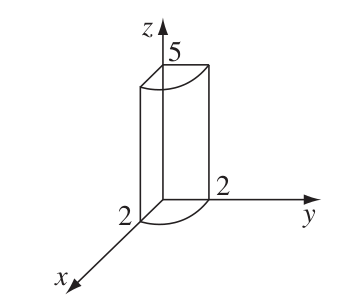
\includegraphics[width=0.3\textwidth]{images/cilindro.png}
    \caption{Coordenadas cilíndricas}
    \label{fig:exemplo}
\end{figure}


Os vetores unitários do sistema cilíndrico são definidos como:

\begin{equation}\label{eq:coor-cilindricas}
\Rightarrow
\begin{cases}
\hat{\mathbf{s}} = \cos\phi \hat{\mathbf{x}} + \sin\phi \hat{\mathbf{y}} \\
\hat{\bm{\phi}} = -\sin\phi \hat{\mathbf{x}} + \cos\phi \hat{\mathbf{y}} \\
\hat{\bm{z}} = \hat{\bm{z}}
\end{cases}
\end{equation}

Determinar $\hat{\mathbf{y}}$ em função $\hat{\mathbf{s}}$ e $\hat{\bm{\phi}}$ em \ref{eq:coor-cilindricas}, podemos multiplicar
por $\sin\phi$ e $\cos\phi$, respectivamente:

\begin{equation}
\mathbf{Somar}
\begin{cases}
    \sin\phi\hat{\mathbf{s}} = \cos\phi\sin\phi \hat{\mathbf{x}} + \sin^{2}\phi \hat{\mathbf{y}}, \\
    \cos\phi\hat{\bm{\phi}} = -\sin\phi\cos\phi \hat{\mathbf{x}} + \cos^{2}\phi \hat{\mathbf{y}}. \\
\end{cases}
\end{equation}

\begin{equation}
    \hat{\mathbf{y}} = \sin\phi \hat{\mathbf{s}} + \cos\phi \hat{\bm{\phi}},
\end{equation}

Agora para $\hat{\mathbf{x}}$, em $\hat{\mathbf{s}}$ e $\hat{\bm{\phi}}$ em \ref{eq:coor-cilindricas}, podemos multiplicar
por $\cos\phi$ e $\sin\phi$, respectivamente:

\begin{equation}
\mathbf{Subtrair}
\begin{cases}
    \cos\phi\hat{\mathbf{s}} = \cos^{2}\phi \hat{\mathbf{x}} + \sin\phi\cos\phi \hat{\mathbf{y}} \\
    \sin\phi\hat{\bm{\phi}} = -\sin^{2}\phi\hat{\mathbf{x}} + \cos\phi \sin\phi \hat{\mathbf{y}} \\
\end{cases}
\end{equation}

\begin{equation}
    \hat{\mathbf{x}} = \cos\phi \hat{\mathbf{s}} - \sin\phi \hat{\bm{\phi}}
\end{equation}

Portanto,

\begin{equation}
    \begin{cases}
        \hat{\mathbf{x}} = \cos\phi \hat{\mathbf{s}} - \sin\phi \hat{\bm{\phi}}, \\
        \hat{\mathbf{y}} = \sin\phi \hat{\mathbf{s}} + \cos\phi \hat{\bm{\phi}}, \\
        \hat{\bm{z}} = \hat{\bm{z}}.
    \end{cases}
    \end{equation}

\section*{Problema 1.44 Griffiths - Resolu\c{c}\~ao}

A função delta de Dirac unidimensional, \(\delta(x)\), pode ser representada como um pico infinitamente alto e 
infinitesimalmente estreito, com área igual a 1. Ou seja:

\begin{equation}
\delta(x) =
\begin{cases}
    0, & \text{se } x \neq 0 \\
    \infty, & \text{se } x = 0
\end{cases}
\end{equation}

e

\begin{equation}
\int_{-\infty}^{\infty} \delta(x) \, dx = 1.
\end{equation}

\begin{equation}
\delta(x-a)=\left\{\begin{array}{ll}
0, & \text { if } x \neq a \\
\infty, & \text { if } x=a
\end{array}\right\} \text { with } \int_{-\infty}^{\infty} \delta(x-a) d x=1
\end{equation}

\begin{equation}
f(x) \delta(x-a)=f(a) \delta(x-a)
\end{equation}

\begin{equation}
\int_{-\infty}^{\infty} f(x) \delta(x-a) d x=f(a)
\end{equation}

Usamos a propriedade da função delta de Dirac:
\begin{equation}
    \int_{a}^{b} f(x) \delta(x - c) dx = f(c), \quad \text{se } c \text{ estiver no intervalo } [a,b].
\end{equation}

(a) \begin{equation}
    \int_{2}^{6} (3x^2 - 2x - 1) \delta(x - 3) dx = 3(3)^2 - 2(3) - 1 = 27 - 6 - 1 = 20.
\end{equation}

(b) Como $\pi \in [0,5]$, temos:
\begin{equation}
    \int_{0}^{5} \cos x \delta(x - \pi) dx = \cos \pi = -1.
\end{equation}

(c) Como $-1 \notin [0,3]$, temos:
\begin{equation}
    \int_{0}^{3} x^3 \delta(x+1) dx = 0.
\end{equation}

(d) Selecionamos $x = -2$:
\begin{equation}
    \int_{-\infty}^{\infty} \ln (x+3) \delta(x+2) dx = \ln(1) = 0.
\end{equation}

\section*{Problema 1.45 Griffiths - Resolu\c{c}\~ao}

(a) Como $\delta(3x) = \frac{1}{3} \delta(x)$:
\begin{equation}
    \int_{-2}^{2} (2x+3) \delta(3x) dx = \frac{1}{3} (2(0) + 3) = \frac{3}{3} = 1.
\end{equation}

(b) Selecionamos $x = 1$:
\begin{equation}
    \int_{0}^{2} (x^3 + 3x + 2) \delta(1 - x) dx = 1^3 + 3(1) + 2 = 6.
\end{equation}

(c) Como $3x + 1 = 0 \Rightarrow x = -1/3$:
\begin{equation}
    \int_{-1}^{1} 9x^2 \delta(3x+1) dx = 9 \left(-\frac{1}{3}\right)^2 \cdot \frac{1}{3} = \frac{1}{3}.
\end{equation}

(d) A integral vale:
\begin{equation}
    \int_{-\infty}^{a} \delta(x - b) dx = \begin{cases} 1, & \text{se } a > b \\ 0, & \text{se } a < b \end{cases}.
\end{equation}

\section*{Problema 1.46 Griffiths - Resolu\c{c}\~ao}


(a) Mostre que:
\begin{equation}
    x \frac{d}{d x} \delta(x)=-\delta(x)
\end{equation}

Vamos come\c{c}ar com:

\begin{equation}
\frac{d}{dx}\left[ xf(x)\delta(x)\right] = \frac{d}{dx}\left( xf(x) \right)\delta(x) + f(x)\left[ x\frac{d}{dx}\delta(x)\right]
\end{equation}

\begin{equation}
    f(x)\left[ x\frac{d}{dx}\delta(x)\right] = \frac{d}{dx}\left[ xf(x)\delta(x)\right] - f(x)\left[ x\frac{d}{dx}\delta(x)\right]
\end{equation}

Integrando ambos os lados sobre o intervalo $[-\infty,\infty]$, temos:


\begin{equation}
    \int_{-\infty}^{\infty} f(x)\left[x \frac{d}{d x} \delta(x)\right] d x=\left.x f(x) \delta(x)\right|_{-\infty} ^{\infty}-\int_{-\infty}^{\infty} \frac{d}{d x}(x f(x)) \delta(x) d x.    
\end{equation}

\begin{equation}
    \int_{-\infty}^{\infty} f(x) \delta(x) d x=0
\end{equation}

\begin{equation}\label{integralderivada}
    \int_{-\infty}^{\infty} f(x)\left[x \frac{d}{d x} \delta(x)\right] d x= -\int_{-\infty}^{\infty} \frac{d}{d x}(x f(x)) \delta(x) d x.    
\end{equation}

\begin{equation}\label{derivadapartes}
    \boxed{
    \frac{d}{d x}(x f(x))=x \frac{d f}{d x}+\frac{d x}{d x} f=x \frac{d f}{d x}+f.
    }
\end{equation}

Usando a equação \ref{derivadapartes} na equação \ref{integralderivada}, temos:

\begin{equation}
    -\int_{-\infty}^{\infty}\left(x \frac{d f}{d x}+f\right) \delta(x) d x=0-f(0)=-f(0)=-\int_{-\infty}^{\infty} f(x) \delta(x) d x
\end{equation}

\begin{equation}
    \int_{-\infty}^{\infty} f(x)\left[x \frac{d}{d x} \delta(x)\right] d x = -\int_{-\infty}^{\infty} f(x) \delta(x) d x
\end{equation}

\begin{equation}
    \int_{-\infty}^{\infty} f(x) \textcolor{red}{\left[x \frac{d}{d x} \delta(x)\right]} d x = \int_{-\infty}^{\infty} f(x)\textcolor{red}{\left[- \delta(x)\right]} d x
\end{equation}

\begin{equation}
    \boxed{
    x \frac{d}{d x} \delta(x)=-\delta(x) \quad \mathbf{qed}
    }
\end{equation}


(b) Mostre que:
\begin{equation}
    \frac{d\theta}{d x} = \delta(x)
\end{equation}

Vamos come\c{c}ar com:

\begin{equation}
\frac{d \theta}{d x}\left[ f(x)\theta(x)\right] = \left[ \frac{d}{dx}f(x)\right]\theta(x) + f(x)\left[ \frac{d \theta}{d x}\right]
\end{equation}

\begin{equation}
    f(x)\left[ \frac{d \theta}{d x}\right] = \frac{d \theta}{d x}\left[ f(x)\theta(x)\right] - \left[ \frac{d}{dx}f(x)\right]\theta(x)
\end{equation}

Integrando ambos os lados sobre o intervalo $[-\infty,\infty]$, temos:

\begin{equation}
    \int_{-\infty}^{\infty} f(x) \frac{d \theta}{d x} d x=\left.f(x) \theta(x)\right|_{-\infty} ^{\infty}-\int_{-\infty}^{\infty} \frac{d f}{d x} \theta(x) d x
\end{equation}


\begin{equation}
    f(\infty)-\int_{0}^{\infty} \frac{d f}{d x} d x=f(\infty)-(f(\infty)-f(0))=f(0)=\int_{-\infty}^{\infty} f(x) \delta(x) d x.
\end{equation}


\begin{equation}
    \int_{-\infty}^{\infty} f(x) \textcolor{red}{\left[\frac{d \theta}{d x}\right]}d x= \int_{-\infty}^{\infty} f(x) \textcolor{red}{\delta(x)} d x.
\end{equation}

\begin{equation}
    \boxed{
    \frac{d \theta}{d x}=\delta(x)
    }
\end{equation}

\section*{Problema 1.47 Griffiths - Resolu\c{c}\~ao}

\begin{enumerate}
    \item[(a)] Escreva uma expressão para a densidade de carga volumétrica $\rho(\mathbf{r})$ de uma 
    carga pontual $q$ na posição $\mathbf{r}'$. Certifique-se de que a integral de volume de $\rho$ 
    resulte em $q$.

    A densidade de carga volumétrica $\rho(\mathbf{r})$ de uma 
    carga pontual $q$ na posição $\mathbf{r}'$, ou seja, definido
    atr\'aves da função delta de Dirac:

    \begin{equation}
        \boxed{\rho(\mathbf{r})=q \delta^{3}\left(\mathbf{r}-\mathbf{r}^{\prime}\right).}
    \end{equation}

    Com a densidade de carga $\rho(\mathbf{r})$ pode calcular a carga total da regi\~ao de interesse,
    fazendo a integra\c{c}\~ao de volume sobre todo o espa\c{c}o:

    \begin{equation}
        \boxed{Q=\int \rho(\mathbf{r}) d \tau=q \int \delta^{3}\left(\mathbf{r}-\mathbf{r}^{\prime}\right) d \tau=q.}
    \end{equation}


    \item[(b)] Qual é a densidade de carga volumétrica de um dipolo elétrico, consistindo em uma 
    carga pontual $-q$ na origem e uma carga pontual $+q$ na posição $\mathbf{a}$?

    \begin{equation}
        \rho(\mathbf{r})=q \delta^{3}(\mathbf{r}-\mathbf{a})-q \delta^{3}(\mathbf{r})
    \end{equation}

    \item[(c)] Qual é a densidade de carga volumétrica (em coordenadas esféricas) de uma casca 
    esférica uniforme, infinitesimalmente fina, com raio $R$ e carga total $Q$, centrada na origem? 
    \textit{(Atenção: a integral sobre todo o espaço deve resultar em $Q$.)}

    \begin{figure}[!h]
    \begin{center}
        \begin{tikzpicture}
            % Desenha a esfera
            \shade[ball color=white!0] (0,0) circle (1);
            
            % Contorno da casca esférica
            \draw[thick] (0,0) circle (1);
            
            % Indicação do raio R
            \draw[->] (0,0) -- (1,0) node[midway, above] {$R$};
            
            % Centro da esfera
            \fill (0,0) circle (1.5pt) node[left] {O};
        \end{tikzpicture}
    \end{center}
    \caption{Casca esférica uniforme com raio $R$ e carga total $Q$.}
    \end{figure}

    Podemos definir a densidade de carga volumétrica como:

    \begin{equation}
        \rho(r)=A \delta(r-R)
    \end{equation}

    Para determinar A precisamos calcular a integra\c{c}\~ao de volume sobre toda a esfera. 
    Usando a formulação de integral de volume de uma esfera:

    \begin{equation}
        Q=\int \rho d \tau=\int A \delta(r-R) 4 \pi r^{2} d r=A 4 \pi R^{2}.
    \end{equation}

    Ent\~ao,

    \begin{equation}
        A=\frac{Q}{4 \pi R^{2}} \rho(r)=\frac{Q}{4 \pi R^{2}} \delta(r-R) .
    \end{equation}

    \begin{equation}
        \boxed{
        \rho(r)=\frac{Q}{4 \pi R^{2}} \delta(r-R) .
        }
    \end{equation}

\end{enumerate}

\section*{Problema 1.48 Griffiths - Resolu\c{c}\~ao}

\begin{enumerate}
    \item[(a)] A função delta de Dirac satisfaz a propriedade de seleção:
    \begin{equation}
    \int f(\mathbf{r}) \delta^3(\mathbf{r} - \mathbf{a}) \, d\tau = f(\mathbf{a}).
    \end{equation}
    Aplicando essa propriedade:
    \begin{equation}
    \int (r^2 + \mathbf{r} \cdot \mathbf{a} + a^2) \delta^3(\mathbf{r} - \mathbf{a}) \, d\tau = a^2 + \mathbf{a} \cdot \mathbf{a} + a^2 = 3a^2.
    \end{equation}

    \item[(b)] Dentro do volume $\mathcal{V}$, que é um cubo centrado na origem, a integral da função delta será não nula apenas se o ponto $\mathbf{b} = 4\hat{\mathbf{y}} + 3\hat{\mathbf{z}}$ estiver dentro do cubo de lado $2$ (ou seja, se $-1 \leq x, y, z \leq 1$). Como $\mathbf{b}$ não está dentro desse intervalo, temos:
    \begin{equation}
    \int_{\mathcal{V}} |\mathbf{r} - \mathbf{b}|^2 \delta^3(5\mathbf{r}) \, d\tau = 0.
    \end{equation}

    \item[(c)] Usamos a propriedade de seleção da delta de Dirac:
    \begin{equation}
    \int_{\mathcal{V}} \left[ r^4 + r^2 (\mathbf{r} \cdot \mathbf{c}) + c^4 \right] \delta^3(\mathbf{r} - \mathbf{c}) \, d\tau.
    \end{equation}
    Como $\mathcal{V}$ é uma esfera de raio $6$ e $\mathbf{c} = 5\hat{\mathbf{x}} + 3\hat{\mathbf{y}} + 2\hat{\mathbf{z}}$, verificamos que o módulo de $\mathbf{c}$ é:
    \begin{equation}
    |\mathbf{c}| = \sqrt{5^2 + 3^2 + 2^2} = \sqrt{25 + 9 + 4} = \sqrt{38} \approx 6.16.
    \end{equation}
    Como $|\mathbf{c}| > 6$, o ponto $\mathbf{c}$ está fora da esfera, então a integral é \textbf{zero}.

    \item[(d)] Similarmente, aplicamos a propriedade da função delta:
    \begin{equation}
    \int_{\mathcal{V}} \mathbf{r} \cdot (\mathbf{d} - \mathbf{r}) \delta^3(\mathbf{e} - \mathbf{r}) \, d\tau.
    \end{equation}
    Avaliamos em $\mathbf{e} = (3,2,1)$:
    \begin{equation}
    \mathbf{e} \cdot (\mathbf{d} - \mathbf{e}) = (3,2,1) \cdot [(1,2,3) - (3,2,1)].
    \end{equation}
    Calculando o vetor diferença:
    \begin{equation}
    \mathbf{d} - \mathbf{e} = (1 - 3, 2 - 2, 3 - 1) = (-2,0,2).
    \end{equation}
    Produto escalar:
    \begin{equation}
    (3,2,1) \cdot (-2,0,2) = 3(-2) + 2(0) + 1(2) = -6 + 0 + 2 = -4.
    \end{equation}
    Como a esfera de raio $1.5$ está centrada em $(2,2,2)$, verificamos se $\mathbf{e} = (3,2,1)$ está dentro dela:
    \begin{equation}
    \sqrt{(3-2)^2 + (2-2)^2 + (1-2)^2} = \sqrt{1^2 + 0^2 + (-1)^2} = \sqrt{2} \approx 1.41.
    \end{equation}
    Como $1.41 < 1.5$, $\mathbf{e}$ está dentro da esfera, então a integral resulta em: -4.
\end{enumerate}

\section*{Problema 1.49 Griffiths - Resolu\c{c}\~ao}

\begin{equation}
J = \int_{\mathcal{V}} e^{-r} \left( \nabla \cdot \frac{\hat{\mathbf{r}}}{r^2} \right) d\tau
\end{equation}

onde $\mathcal{V}$ é uma esfera de raio $R$, centrada na origem, utilizando dois métodos diferentes, como no Ex. 16.

Vamos utilizar a equação 1.99 (Griffiths, quarta edição) para calcular a integral:
\begin{equation}
    \nabla\cdot \left(\frac{\hat{\mathbf{r}}}{r^2}\right) = 4\pi \delta^{3}(\mathbf{r})
\end{equation}

\begin{equation}
    J=\int e^{-r}\left(4 \pi \boldsymbol{\delta}^{3}(\mathbf{r})\right) d \tau=4 \pi e^{-0}=4 \pi \quad \checkmark
\end{equation}

ou com equação 1.59 para calcular a integra\c{c}\~ao por partes:

\begin{equation}
\int_{\mathcal{V}} f \left( \nabla \cdot \mathbf{A} \right) d\tau = -\int_{\mathcal{V}}\mathbf{A} \cdot (\nabla f)\, d\tau + \oint_S f \mathbf{A} \cdot d\mathbf{a}.
\end{equation}

Como isso, temos:

\begin{equation}
    \int_{\mathcal{V}} e^{-r} \left( \nabla \cdot \frac{\hat{\mathbf{r}}}{r^2} \right) d\tau = -\int_{\mathcal{V}}\frac{\hat{\mathbf{r}}}{r^2} \cdot (\nabla (e^{-r}))\, d\tau + \oint_S (e^{-r}) \frac{\hat{\mathbf{r}}}{r^2} \cdot d\mathbf{a},
\end{equation}

Logo, a integral da $J$:

\begin{equation}
    J = \int_{\mathcal{V}} e^{-r} \left( \nabla \cdot \frac{\hat{\mathbf{r}}}{r^2} \right) d\tau = -\int_{\mathcal{V}}\frac{\hat{\mathbf{r}}}{r^2} \cdot (\nabla (e^{-r}))\, d\tau + \oint_S (e^{-r}) \frac{\hat{\mathbf{r}}}{r^2} \cdot d\mathbf{a}.
\end{equation}

\[
J = -\int_{\mathcal{V}} \frac{\hat{\mathbf{r}}}{r^2} \cdot \nabla (e^{-r}) \, d\tau + \oint_{\mathcal{S}} e^{-r} \frac{\hat{\mathbf{r}}}{r^2} \cdot d\mathbf{a}.
\]
Mas 
\[
\nabla (e^{-r}) = \left( \frac{\partial}{\partial r} e^{-r} \right) \hat{\mathbf{r}} = -e^{-r} \hat{\mathbf{r}}.
\]

\[
= \int_0^R \frac{1}{r^2} e^{-r} 4\pi r^2 \, dr + \int e^{-R} \frac{\hat{\mathbf{r}}}{r^2} \cdot r^2 \sin\theta \, d\theta \, d\phi \, \hat{\mathbf{r}}
\]

\[
= 4\pi \int_0^R e^{-r} \, dr + e^{-R} \int \sin\theta \, d\theta \, d\phi
\]

\[
= 4\pi \left( -e^{-r} \right) \Big|_0^R + 4\pi e^{-R} = 4\pi (-e^{-R} + e^{0}) + 4\pi e^{-R} = 4\pi. \quad \checkmark
\]

\[
(\text{Aqui } R = \infty, \text{ logo } e^{-R} = 0.)
\]


\section*{Problema 1.51 Griffiths - Resolu\c{c}\~ao}

\begin{itemize}
    \item[(d) $\Rightarrow$ (a):] $\nabla \times \mathbf{F} = \nabla \times (-\nabla U) = 0 \quad (\text{Eq. 1.44 – curl of gradient is always zero}).$
    \item[(a) $\Rightarrow$ (c):] $\oint \mathbf{F} \cdot d\mathbf{l} = \int (\nabla \times \mathbf{F}) \cdot d\mathbf{a} = 0 \quad (\text{Eq. 1.57 – Stokes’ theorem}).$
    \item[(c) $\Rightarrow$ (b):] $\int_a^b \mathbf{F} \cdot d\mathbf{l} - \int_a^b \mathbf{F}_{II} \cdot d\mathbf{l} = \int_a^b \mathbf{F} \cdot d\mathbf{l} + \int_b^a \mathbf{F}_{II} \cdot d\mathbf{l} = \oint \mathbf{F} \cdot d\mathbf{l} = 0,$ 
    so 
    \[
    \int_a^b \mathbf{F} \cdot d\mathbf{l} = \int_a^b \mathbf{F}_{II} \cdot d\mathbf{l}.
    \]
    \item[(b) $\Rightarrow$ (c):] same as (c) $\Rightarrow$ (b), only in reverse; 
    \item[(c) $\Rightarrow$ (a):] same as (a) $\Rightarrow$ (c).
\end{itemize}

\section*{Problema 1.52 Griffiths - Resolu\c{c}\~ao}

\begin{itemize}
    \item[(d) $\Rightarrow$ (a):] $\nabla \cdot \mathbf{F} = \nabla \cdot (\nabla \times \mathbf{W}) = 0 \quad (\text{Eq. 1.46 – divergence of curl is always zero}).$
    \item[(a) $\Rightarrow$ (c):] $\oint \mathbf{F} \cdot d\mathbf{a} = \int (\nabla \cdot \mathbf{F}) \, d\tau = 0 \quad (\text{Eq. 1.56 – divergence theorem}).$

    (c) $\Rightarrow$ (b): \(\int_I \mathbf{F} \cdot d\mathbf{a} - \int_{II} \mathbf{F} \cdot d\mathbf{a} = \oint \mathbf{F} \cdot d\mathbf{a} = 0,\) so  
\[
\int_I \mathbf{F} \cdot d\mathbf{a} = \int_{II} \mathbf{F} \cdot d\mathbf{a}.
\]

\textit{(Note: sign change because for} \(\oint \mathbf{F} \cdot d\mathbf{a}\), \textit{da is} \textit{outward}, \textit{whereas for surface II it is} \textit{inward}.)  

(b) $\Rightarrow$ (c): same as (c) $\Rightarrow$ (b), in reverse; (c) $\Rightarrow$ (a): same as (a) $\Rightarrow$ (c).

\end{itemize}

\section*{Problema 1.62 Griffiths - Resolu\c{c}\~ao}

\begin{itemize}
    \item[(a)] $d\mathbf{a} = R^2 \sin \theta \, d\theta \, d\phi \, \hat{\mathbf{r}}.$ Let the surface be the northern hemisphere. The $\hat{\mathbf{x}}$ and $\hat{\mathbf{y}}$ components clearly integrate to zero, and the $\hat{\mathbf{z}}$ component of $\hat{\mathbf{r}}$ is $\cos \theta$, so  
    \[
    \mathbf{a} = \int R^2 \sin \theta \cos \theta \, d\theta \, d\phi \, \hat{\mathbf{z}}
    = 2\pi R^2 \hat{\mathbf{z}} \int_0^{\pi/2} \sin \theta \cos \theta \, d\theta 
    = 2\pi R^2 \hat{\mathbf{z}} \left.\frac{\sin^2 \theta}{2}\right|_0^{\pi/2} 
    = \pi R^2 \hat{\mathbf{z}}.
    \]

    \item[(b)] Let $T = 1$ in Prob. 1.61(a). Then $\nabla T = 0$, so $\oint d\mathbf{a} = 0.$ \hspace{1cm} qed

    \item[(c)] This follows from (b). For suppose $\mathbf{a}_1 \neq \mathbf{a}_2$; then if you put them together to make a closed surface, 
    \[
    \oint d\mathbf{a} = \mathbf{a}_1 - \mathbf{a}_2 \neq 0.
    \]

    \item[(d)] For one such triangle, $d\mathbf{a} = \frac{1}{2} (\mathbf{r} \times d\mathbf{l})$ (since $\mathbf{r} \times d\mathbf{l}$ is the area of the parallelogram, and the direction is perpendicular to the surface), so for the entire conical surface, 
    \[
    \mathbf{a} = \frac{1}{2} \oint \mathbf{r} \times d\mathbf{l}.
    \]

    \item[(e)] Let $T = \mathbf{c} \cdot \mathbf{r}$, and use product rule \#4: 
    \[
    \nabla T = \nabla (\mathbf{c} \cdot \mathbf{r}) = \mathbf{c} \times (\nabla \times \mathbf{r}) + (\mathbf{c} \cdot \nabla)\mathbf{r}.
    \] 
    But $\nabla \times \mathbf{r} = 0$, and $(\mathbf{c} \cdot \nabla)\mathbf{r} = (c_x \frac{\partial}{\partial x} + c_y \frac{\partial}{\partial y} + c_z \frac{\partial}{\partial z})(x \hat{\mathbf{x}} + y \hat{\mathbf{y}} + z \hat{\mathbf{z}}) = c_x \hat{\mathbf{x}} + c_y \hat{\mathbf{y}} + c_z \hat{\mathbf{z}} = \mathbf{c}.$  
    So Prob. 1.61(e) says  
    \[
    \oint T \, d\mathbf{l} = \oint (\mathbf{c} \cdot \mathbf{r}) \, d\mathbf{l} = -\int (\nabla T) \times d\mathbf{a} = -\int \mathbf{c} \times d\mathbf{a} = -\mathbf{c} \times \mathbf{a} = \mathbf{a} \times \mathbf{c}.
    \]
    \hspace{1cm} qed
\end{itemize}


\section*{Problema 1.63 Griffiths - Resolu\c{c}\~ao}

\begin{equation}
    \nabla \cdot \mathbf{v}=\frac{1}{r^{2}} \frac{\partial}{\partial r}\left(r^{2} \cdot \frac{1}{r}\right)=\frac{1}{r^{2}} \frac{\partial}{\partial r}(r)=\frac{1}{r^{2}} .
\end{equation}
    
Para uma esfera de raio $R$ :

\begin{equation}
\left.\begin{array}{rl}
\int \mathbf{v} \cdot d \mathbf{a} & =\int\left(\frac{1}{R} \hat{\mathbf{r}}\right) \cdot\left(R^{2} \sin \theta d \theta d \phi \hat{\mathbf{r}}\right)=R \int \sin \theta d \theta d \phi=4 \pi R . \\\
(\nabla \cdot \mathbf{v}) d \tau & =\int\left(\frac{1}{r^{2}}\right)\left(r^{2} \sin \theta d r d \theta d \phi\right)=\left(\int_{0}^{R} d r\right)\left(\int \sin \theta d \theta d \phi\right)=4 \pi R .
\end{array}\right\} \begin{aligned}
& {*}\\
& 
\end{aligned}
\end{equation}

*Portanto, o teorema da divergência está verificado.

Evidentemente, não há uma função delta na origem.

\begin{equation}
\nabla \times\left(r^{n} \hat{\mathbf{r}}\right)=\frac{1}{r^{2}} \frac{\partial}{\partial r}\left(r^{2} r^{n}\right)=\frac{1}{r^{2}} \frac{\partial}{\partial r}\left(r^{n+2}\right)=\frac{1}{r^{2}}(n+2) r^{n+1}=(n+2) r^{n-1}
\end{equation}

exceto para $n=-2$, para o qual já sabemos (Eq. 1.99) que a divergência é $4 \pi \delta^{3}(\mathbf{r})$.

(2) Geometricamente, deve ser zero. Da mesma forma, o rotacional em coordenadas esféricas obviamente resulta em zero. 
Para garantir que não há uma função delta oculta, integramos sobre uma esfera de raio $R$, usando o Problema 1.61(b): 
Se 

\begin{equation}
    \nabla \times\left(r^{n} \hat{\mathbf{r}}\right)=\mathbf{0}
\end{equation}

então
\begin{equation} 
\int(\nabla \times \mathbf{v}) d \tau=\mathbf{0} \stackrel{?}{=} \circ \mathbf{v} \times d \mathbf{a} 
\end{equation}

Mas 

\begin{equation}
    \mathbf{v}=r^{n} \hat{\mathbf{r}}
\end{equation}

e 

\begin{equation}
    d \mathbf{a}=R^{2}\sin \theta d \theta d \phi \hat{\mathbf{r}}
\end{equation}

estão ambos na direção de $\hat{\mathbf{r}}$, logo:
\begin{equation}
\mathbf{v} \times d \mathbf{a}=\mathbf{0} . \checkmark
\end{equation}

%%%%%%%% Bibliography 
% Os comandos para incluir as referências bibliográficas
%\printingbibliography

\end{document}
